%
% 3dimagetemplate.tex
%
% (c) 2021 Prof Dr Andreas Müller, OST Ostschweizer Fachhochschule
%
\documentclass[tikz]{standalone}
\usepackage{times}
\usepackage{amsmath}
\usepackage{txfonts}
\usepackage[utf8]{inputenc}
\usepackage{graphics}
\usetikzlibrary{arrows,intersections,math}
\usepackage{ifthen}
\begin{document}

\newboolean{showgrid}
\setboolean{showgrid}{false}
\def\breite{7}
\def\hoehe{9}

\begin{tikzpicture}[>=latex,thick]
\begin{scope}
\clip (-6.3,-9.1) rectangle (6.3,9.1);

% Povray Bild
\node at (0,5.45) {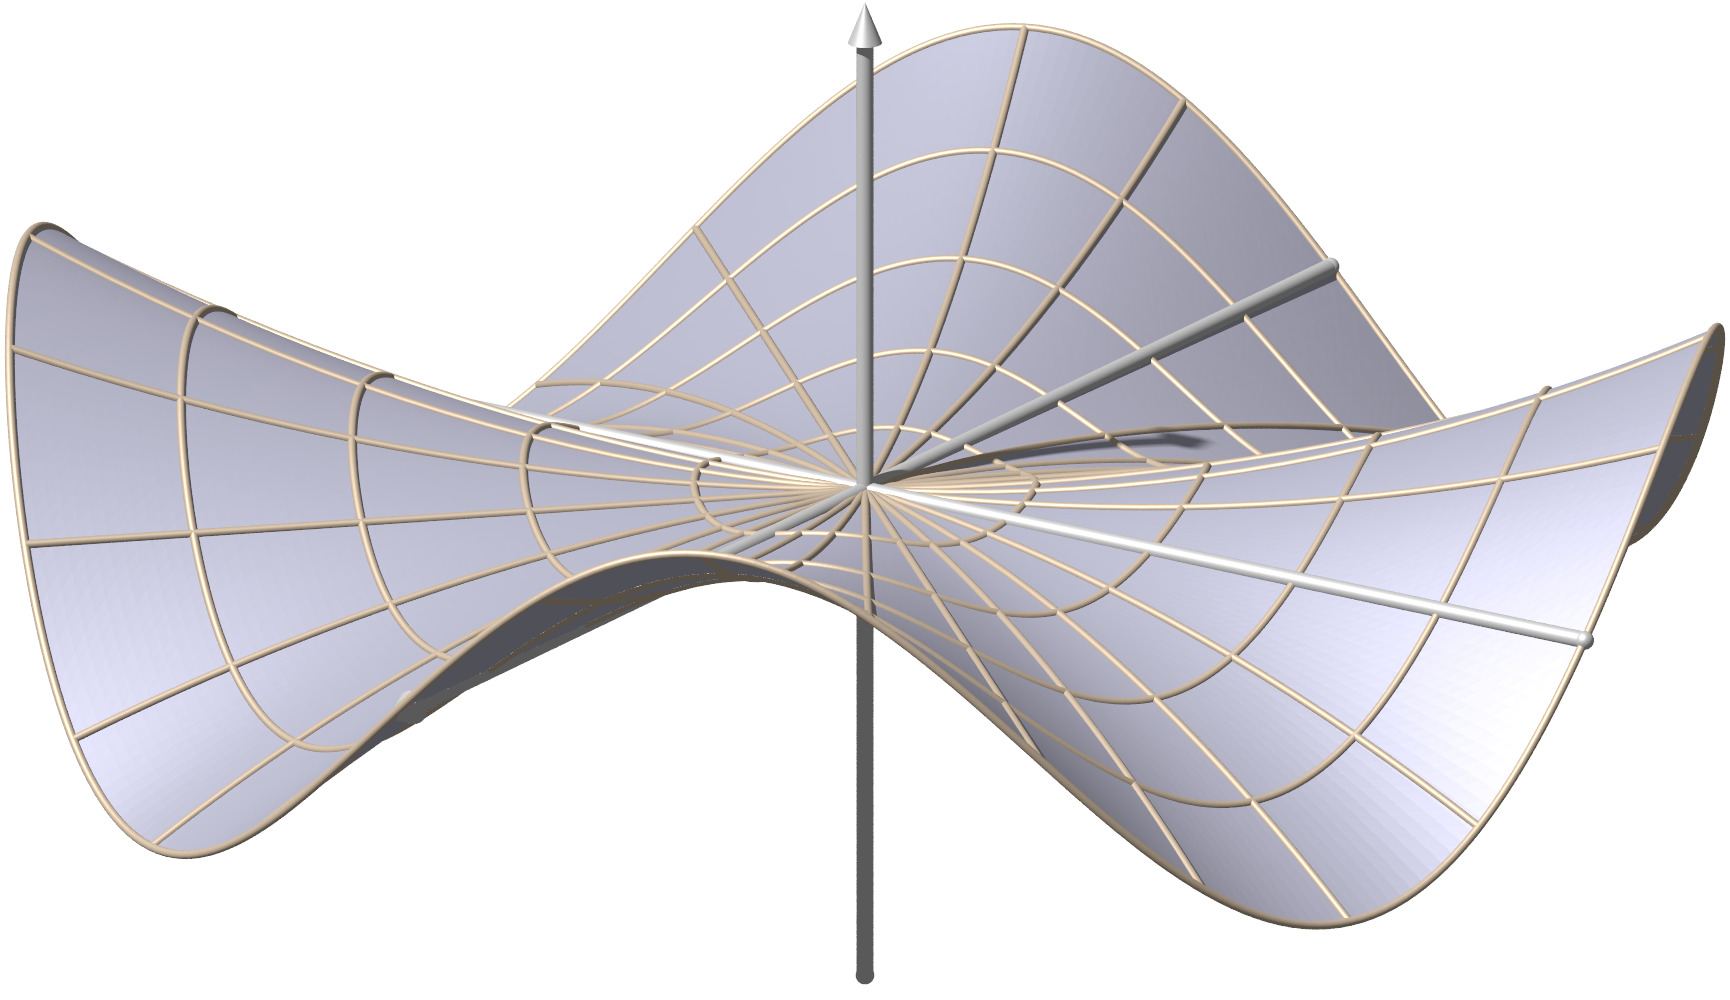
\includegraphics[width=12.6cm]{schwarz.jpg}};
\node at (0,-5.45) {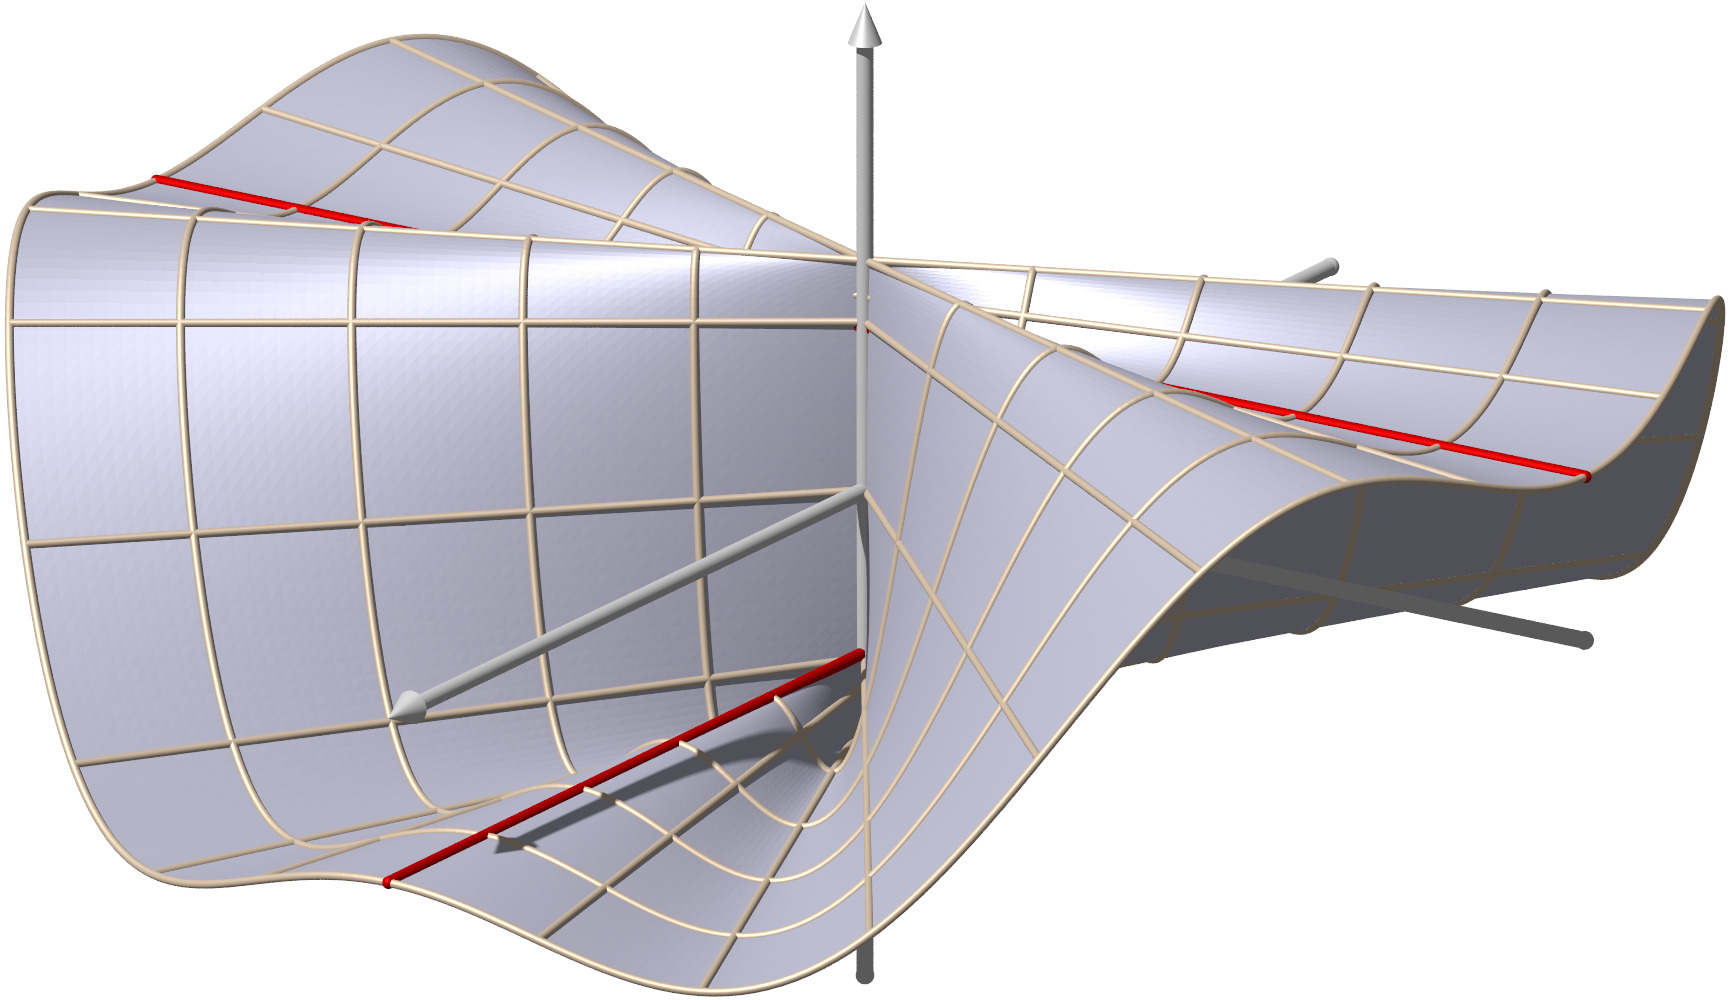
\includegraphics[width=12.6cm]{schwarzxy.jpg}};
\node at (-3.2,0) {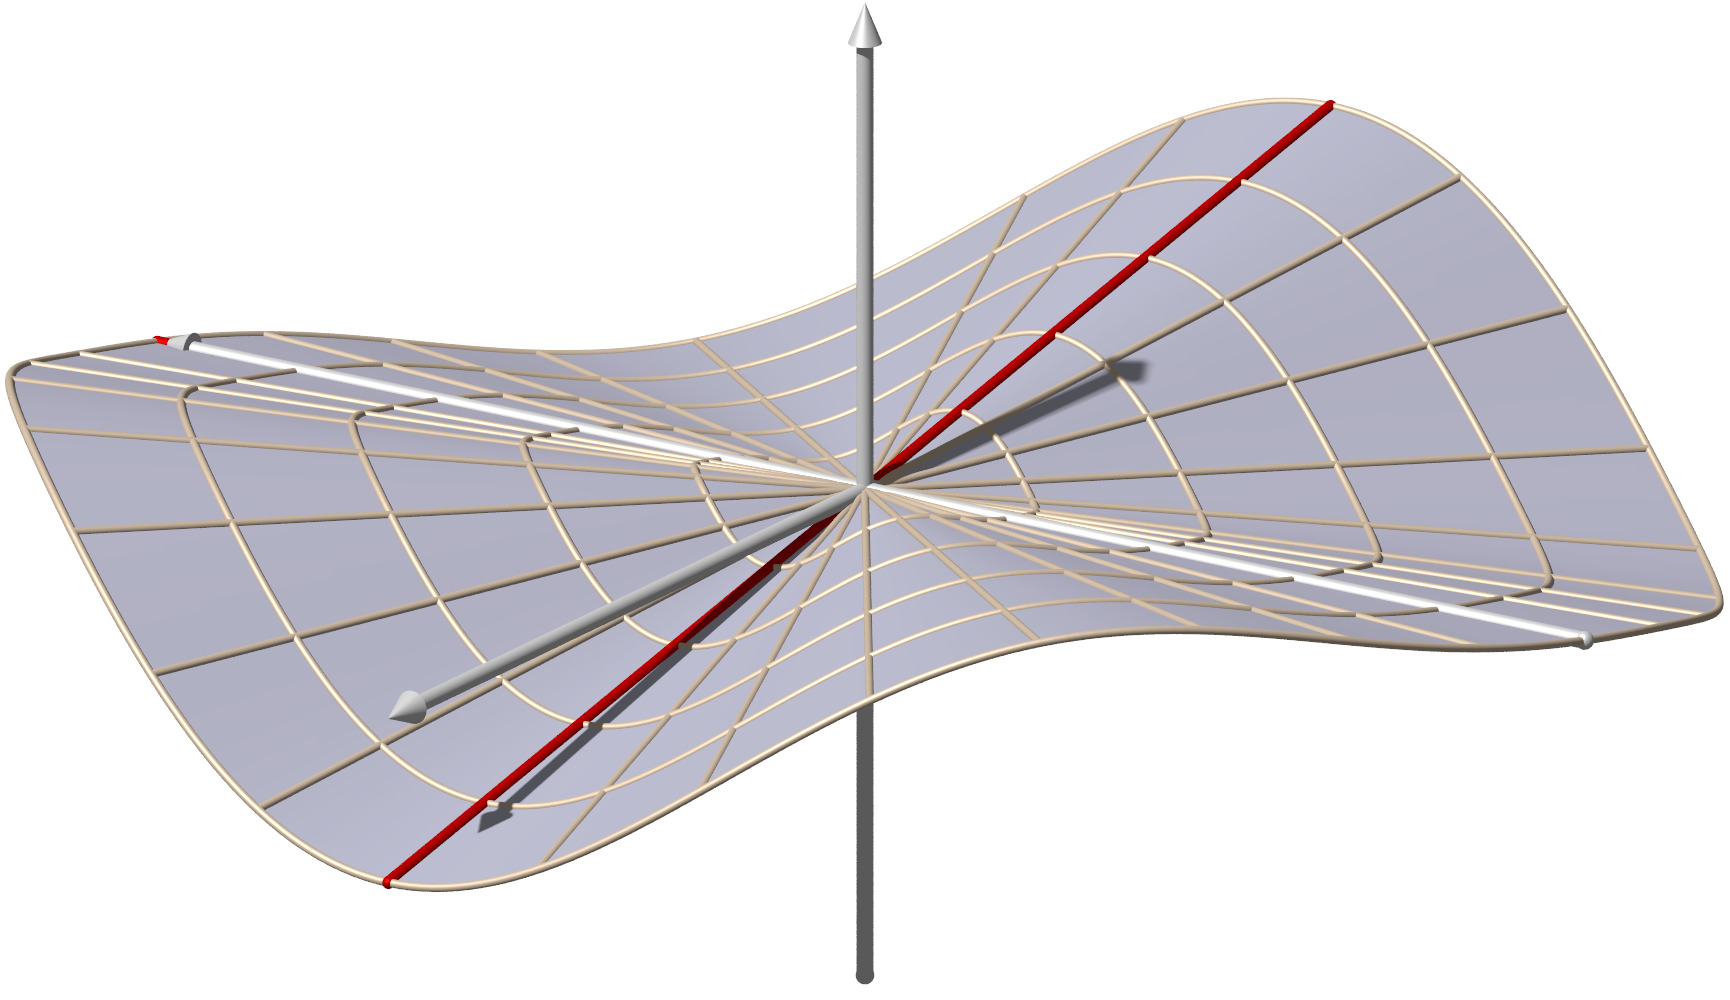
\includegraphics[width=6.1cm]{schwarzx.jpg}};
\node at (3.2,0) {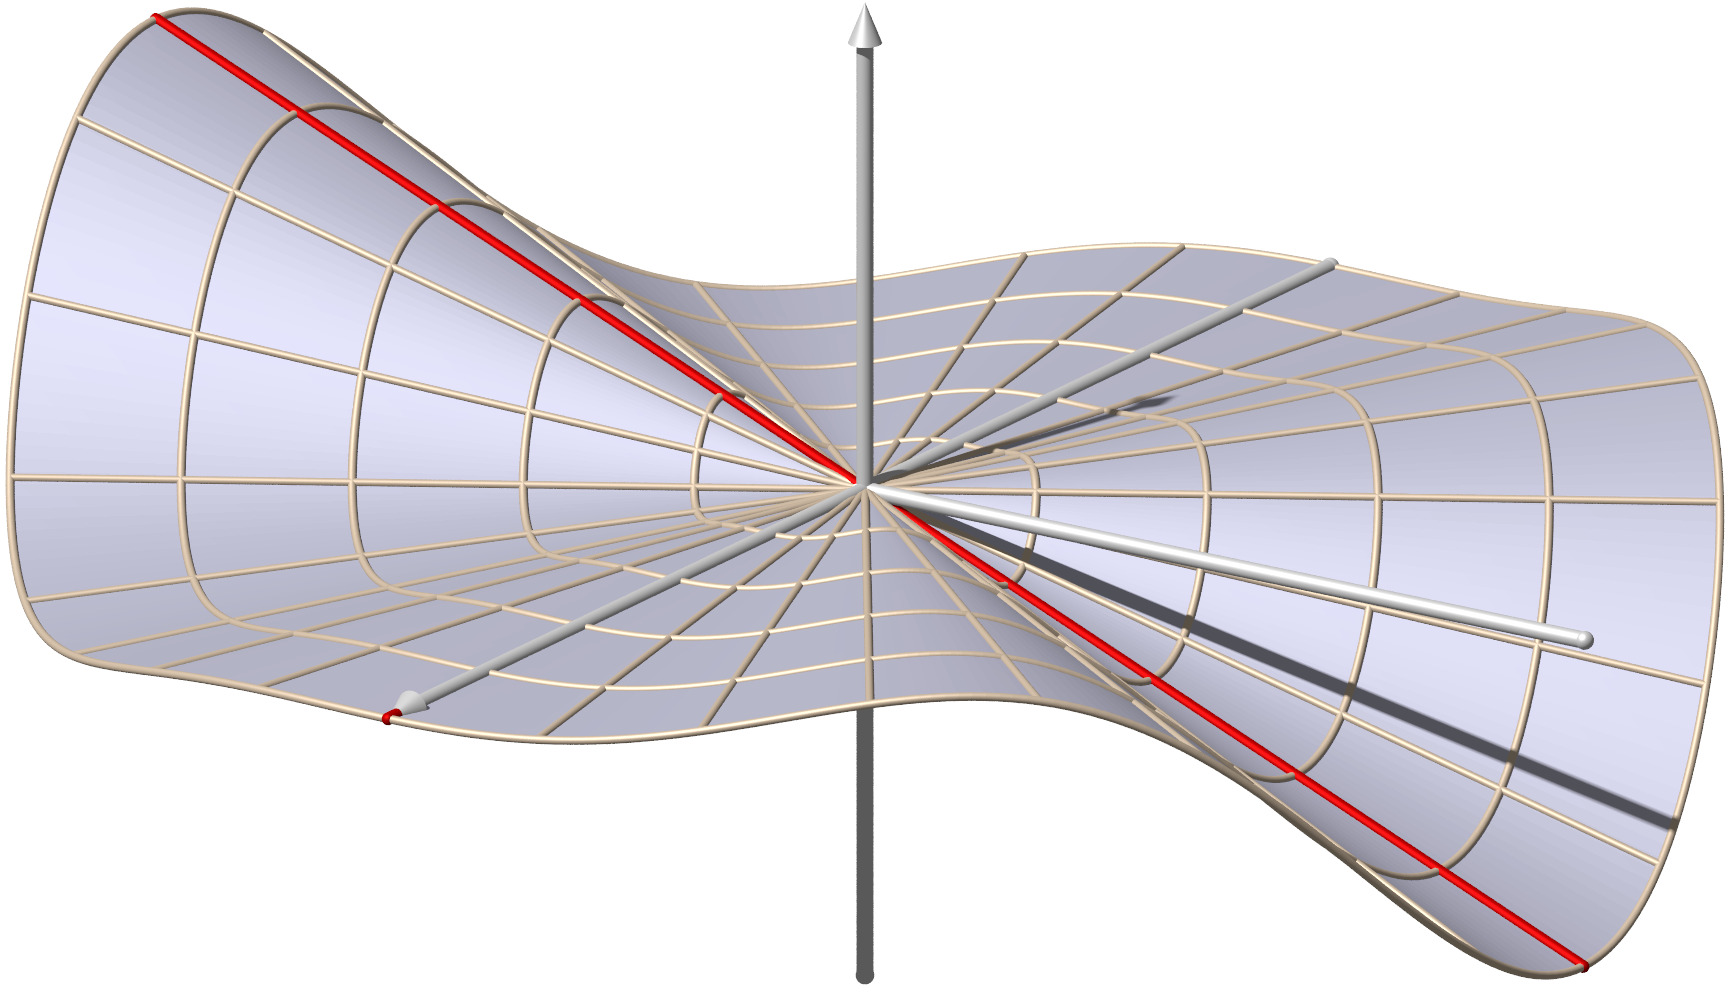
\includegraphics[width=6.1cm]{schwarzy.jpg}};

\end{scope}

% Gitter
\ifthenelse{\boolean{showgrid}}{
\draw[step=0.1,line width=0.1pt] (-\breite,-\hoehe) grid (\breite, \hoehe);
\draw[step=0.5,line width=0.4pt] (-\breite,-\hoehe) grid (\breite, \hoehe);
\draw                            (-\breite,-\hoehe) grid (\breite, \hoehe);
\fill (0,0) circle[radius=0.05];
}{}

\begin{scope}
\clip (-6.3,-9.1) rectangle (6.3,9.1);

% f
\node at (-4,8) {$\displaystyle
	z = f(x,y) = \frac{x^3y-xy^3}{x^2+y^2}
	$};
\node at (-0.3,8.9) {$z\mathstrut$};
\node at (5.5,4.3) {$-y\mathstrut$};
\node at (-3.4,4.2) {$x\mathstrut$};

% fx
\node at (-5.3,1.5) {$\displaystyle
	z=\frac{\partial f}{\partial x\mathstrut}(x,y)
	$};
\node at (-4.9,-0.6) {$x\mathstrut$};
\node at (-5.7,0.8) {$y\mathstrut$};
\node at (-3.4,1.7) {$z\mathstrut$};

% fy
\node at (5.3,1.5) {$\displaystyle
	z=\frac{\partial f}{\partial y\mathstrut}(x,y)
	$};
\node at (1.5,-1.0) {$x\mathstrut$};
\node at (5.7,-0.4) {$-y\mathstrut$};
\node at (3.0,1.7) {$z\mathstrut$};

% fxy
\node at (5.0,-3.0) {$\displaystyle z=
	\frac{\partial^2 f}{\partial x\,\partial y}(x,y)
	$};
\node at (5.4,-6.7) {$-y\mathstrut$};
\node at (-3.4,-6.7) {$x \mathstrut$};
\node at (-0.3,-2) {$z\mathstrut$};

\end{scope}

\end{tikzpicture}

\end{document}

